\normalfont\normalsize

\chapter{Static scheduling}

A first step in task scheduling would be to consider the static case, where all the tasks that have to run are known from the beginning. An
assignment to nodes would take place, then the results will be distributed to the nodes. The system will not allow at first the adding
or removal of tasks. This static case will have a more efficient scheduling because of its conditions, so it is to be preferred to the dynamic
one if we already have all the prerequisites.  Indeed most applications will be a mixture of static and dynamic functionalities, so the tasks
belonging to the former will be scheduled in the beginning, more efficiently, then the one from the latter will be scheduled as need arises.

\section{Assumptions}

We have discussed the hardware and software platform, and now we must note some characteristics of how they relate to the scheduling problem.
First of all the network in this phase can only have star topology, as this is all that supports Contiki's UIP stack. Only the Raven USB stick 
with Contiki can act as a router. This is not very relevant as behaviour in a larger, multi-hop network relies on this basic star topology.  One
important feature is that nodes can send messages to one another directly. 

When we will measure the energy consumed running a task we will consider that energy consumed in idle time is negligeble. However, Contiki does not
have any power management on the stack level, so power is wasted even in idle state. This should not affect the results on the scheduling algorithm,
as the energy relevant to the problem is taken into account.

Some nodes have extra peripherals attached, such as LCDs or LEDs or speakers. This will appear as extra consumption on these nodes, so the scheduler
will not favor them as much when choosing an appropriate node for a task. This is not a problem, on the contrary, it should demonstrate the usefulness
of the scheduler in a heterogenous wireless network.

\section{Energy considerations}

Energy efficiency is a key issue in WSN applications and is no stranger to this study. WSNs have limited, irreplaceable energy sources (most of the time,
wireless nodes that incorporate any form of energy harvesting take exception from this fact) but have harsh lifetime requirements. In order to formulate 
criteria for scheduling to minimize energy consumption, we have to discuss how energy is consumed in a WSN. 

The main culprit in energy consumption is radio communication. Energy spent on time communicating on wireless is about a couple of hundreds up to a thousand times
larger than the energy spent processing on the microcontroller. Thus energy savings efforts must go into keeping the wireless chip in low-power states as much as possible.

Another interesting fact is transmission versus reception power. Both in the transmit state and the receive state, the RF part of the transceiver is active, so it may
seem that the two are energy-equivalent. However, due to differences in hardware design, the transceiver will consume more power in the receive state. Although 
transmission times are kept low because transmission generally occurs in small bursts, the nodes must be able to receive messages at all times. Even if a proper
communicating schedule is put in place, receive timer will still be much larger.

Channel sensing, to be used in CSMA (Carrier Sensing Multiple Access), has about the same energy requirements as receiving and transmitting, making MAC protocols that abuse
it energy inefficient.

Energy savings could be done with power control over the transceiver, reducing the detection and communication radii. 
However, this only reduces power consumption at almost half the initial value, which is not considered to be a relevant
energy saving in respect to the need to put a lot more nodes to compensate for the small radius of communication. 


\section{Problem Definition}
\label{sec:problem}

The problem we address is an unconventional scheduling algorithm, in the sense that the main constraint is not time, but energy. As shown in Related
Work, research on scheduling is generally focused on hard time deadlines. Instead, we propose a solution where time is of least importance, preceded 
by energy consumption, battery awareness, availability and affinity.

The task that we wish to schedule is the smallest indivisible part of an application. Tasks can be classified into sensing tasks, actuating tasks,
detection tasks, etc. For example, we have a fire detection system implemented with a WSN. We can have smoke sensing tasks on nodes that have smoke sensors,
an event detection task, that detects in a stream of sensor input when smoke levels have risen, and an alarm task, that handles the behaviour of the
network in the case of fire (bell, speaker, opening doors, etc.).  

For the previous scenario, the scheduler needs some basic information for each task: its importance, an affinity to a certain type of node (a smoke sensing
task can only be assigned to wireless nodes that have a smoke sensor), a frequency with which to run (most if not all tasks in a WSN are repeteable) and
data sinks (addresses and ports). In the fire detection scenario, one setup can be the following: some nodes can have smoke sensing tasks 
with a certain frequency (e.g. once every minute),\footnote{A variation of the algorithm that takes into account low-battery states for nodes or just 
where a task can't be scheduled due to network overencumbrance can be implemented, similar to\cite{Deli2005}}
situations the tasks have a single data sink (different from the gateway) on a node that does not have a smoking
sensor. The event detection task is assigned on that node, it runs an algorithm on the data received from all the nodes and determines if there's a fire 
and where it would be. The output of this task is handed over to nodes that handle the alarm (multiple data sinks for this task).  Each node that has
an alarm or actuates a device in case of fire is registered with that event detection task. When it receives positive confirmation of a fire, it triggers
the alarm. 

\begin{table}[htb]
 \centering
\begin{tabular}{|l|c|c|}
\hline
Parameter & Before scheduling & After scheduling\\
\hline
Importance & \tick & \\
\hline
Data sinks &	&  \tick\\
\hline
Frequency  & \tick & \tick\\
\hline
Node Affinity & \tick & \\
\hline
Multiplicity & \tick & \tick\\
\hline
Data dependency & \tick & \\
\hline
\end{tabular}
\caption{Origin of task properties}
\label{tab:origin}

\end{table}

This setup is scalable, meaning there can be more than one node running the event detection task, assuring minimal energy consumption. So another
parameter for a task that has to be scheduled is its multiplicity, which can be a number or left to the scheduler to adjust\footnote{
Another possible variation of the algorithm is when the number of task to run in the network is determined by the scheduler itself. The ultimate goal
of the application needs to be taken into account, and some tasks are better left to run on more nodes for the sake of the application or of energy
awareness}. Data dependencies between these types of tasks (smoke sensing, event detection and alarm) should be clear from the start.

To summarize, the properties of a task and the moments when they can be determined are shown in Table \ref{tab:origin}. 
Notice that some can be determined in both moments, according to the variation of the algorithm. 



Thus the problem is to schedule a number of tasks, having the WSN and its topology as input, and the tasks' frequencies and data dependencies. The 
scheduler finds the best assignment that maximizes network lifetime and achieves the application goal. Results are evaluated by calculating the total
energy cost of the tasks running in the WSN.

\section{Initial Metrics}

\subsection{Battery Level}

The first important metric that needs to be taken into account when scheduling tasks is battery status. We will use the 
Atmega Analog to Digital Converter (ADC) for this purpose, however this cannot be accomplished by measuring the ADC0 
pin on the Atmega3290 on the Raven board, because there is a reference voltage of either 1.1V (internal) or VCC, so it 
will always read maximum. The solution is to connect the power supply to one of the voltage 
measurement inputs, one that already has a voltage divider, which is connected to the ADC3 pin.
\[ADC_3 = \frac{100K}{471K} \cdot VCC\;<VCC\]
\begin{figure}[ht]
 \begin{center}
  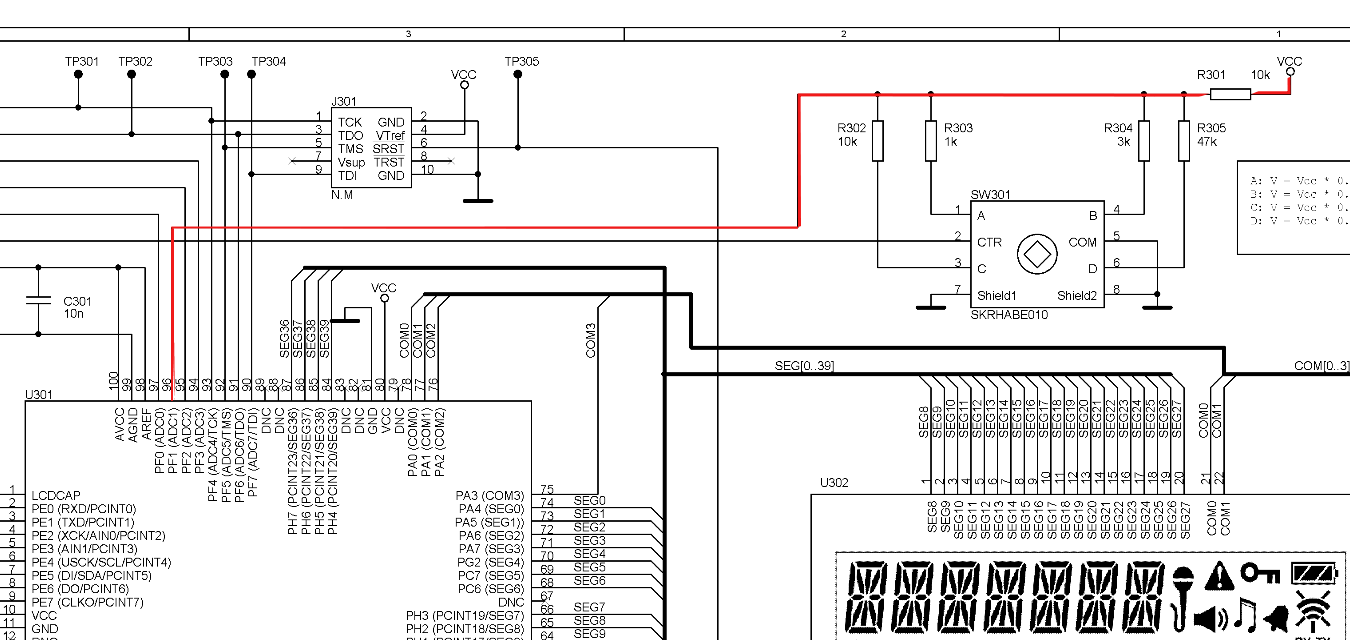
\includegraphics{static/adc0.png}
 \end{center}
  \caption{\small \itshape{$ADC0$ voltage measurement highlighted on the AVR Raven schematic}}

\end{figure}

The ADC is available only on the Atmega3290 microcontroller so the information has to be transferred to the Atmega1284. This is done once every 10
seconds, when the Atmega3290 sends a frame (Contiki has an additional communication layer on top of the existing inter-processor USART) with a
SET\_BATT command, and with a unsigned 16-bit integer as payloadi (broken into bytes). The integer sent is exactly the ADC conversion result, 
right-aligned (only the 10 least significant bits are used). The integer is recomposed at the other end and saved in the data memory. We will discuss
later how this information reaches the scheduler service. The battery indicator on the display LCD of the Raven board is also used to display status. 

\begin{figure}[ht]
 \begin{center}
  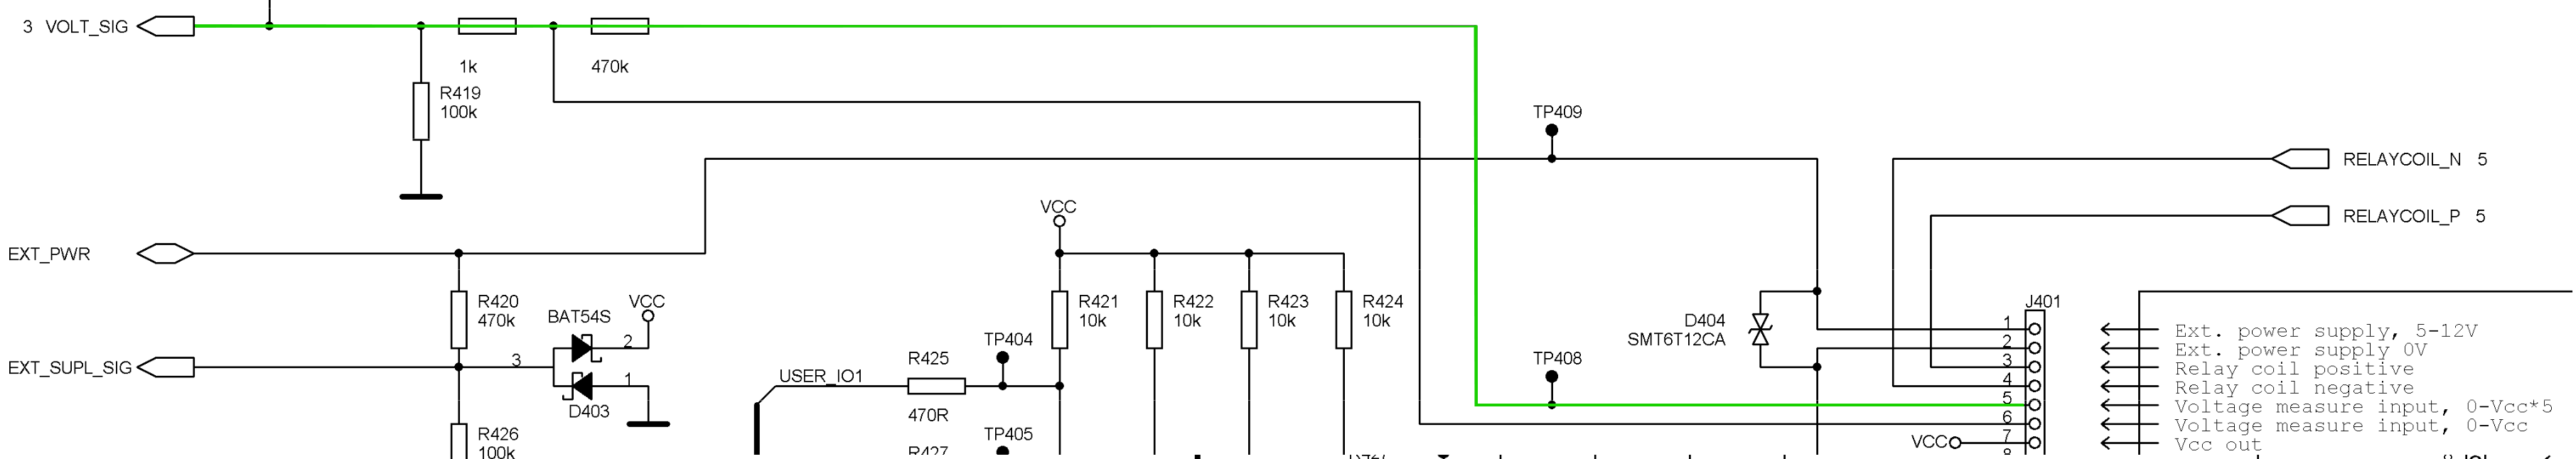
\includegraphics[scale=0.86]{static/voltsig.png}
 \end{center}
  \caption{\small \itshape{$ADC3$ voltage measurement through voltage divider on PCB highlighted on the AVR Raven schematic}}

\end{figure}
\subsection{Node affinity}

In this section we define the \textit{Node affinity} for our scheduler: Each task can only run on certain nodes, as was previously discussed. 
For this reason we create the affinity parameter, which is $0$ for assignments $(v,m)$ (task $v$ and node $m$) 
that are imcompatible and $1$ for compatible assignments.
We might also define this notion from the nodes' point of view. which further illustrates the connection between Node Affinity and its implementation:
Each sensor node has a specific set of capabilities: It can run sensing tasks based on attached sensors, or actuating tasks that are compatible with
actuators attached, diverse computing tasks and so on. 

This is implemented on the platform by compiling into the board code some Contiki processes, while others
are left out. This means that each node is aware of the processes it contains, and can advertise that to the scheduler. What happens is that each node
will have several \textit{metaprocesses}, processes that help the scheduling, know which processes exist on a node and can start them upon command.
One of these processes will advertise to the scheduler (to the network node on which the scheduler runs, in this case a PC) the node parameters,
its battery status and capabilities.

Let $C_m$ be the set of capabilities advertised by a sensor node. Each task has a set of capabilities needed in order to run (a smoke sensor for a smoke
sensing task), let this be $C_v$. Node affinity in the case of a possible assignment $(v,m)$ is $1$ if $C_v\, \subset\,C_m$, and $0$ otherwise. Node affinity
for a task (not an assignment) will be the set of nodes $M$, such that $\forall m_i\,\epsilon\,M,\: NA((v,m))=1$, where $NA((v,m))$ is Node Affinity for
the assignment of task $v$ to node $m$.


\subsection{Node load}
\label{sec:nodeload}


As described in \ref{sec:contikitask} we can measure node load by looking at the time between schedules of the same dummy-task. This is especially
useful when dealing with processing tasks outside the task context. However, the tasks are periodic so they only run when their event timer expires.
Then the metric would be reduced to showing the number of processes actively running and processing. This has to be combined with a normal calculation
of tasks and their frequencies to tell if a node can run another task or not.

\section{Assessment Metrics}
\label{sec:metrics}

\begin{figure}[ht]
 \begin{center}
  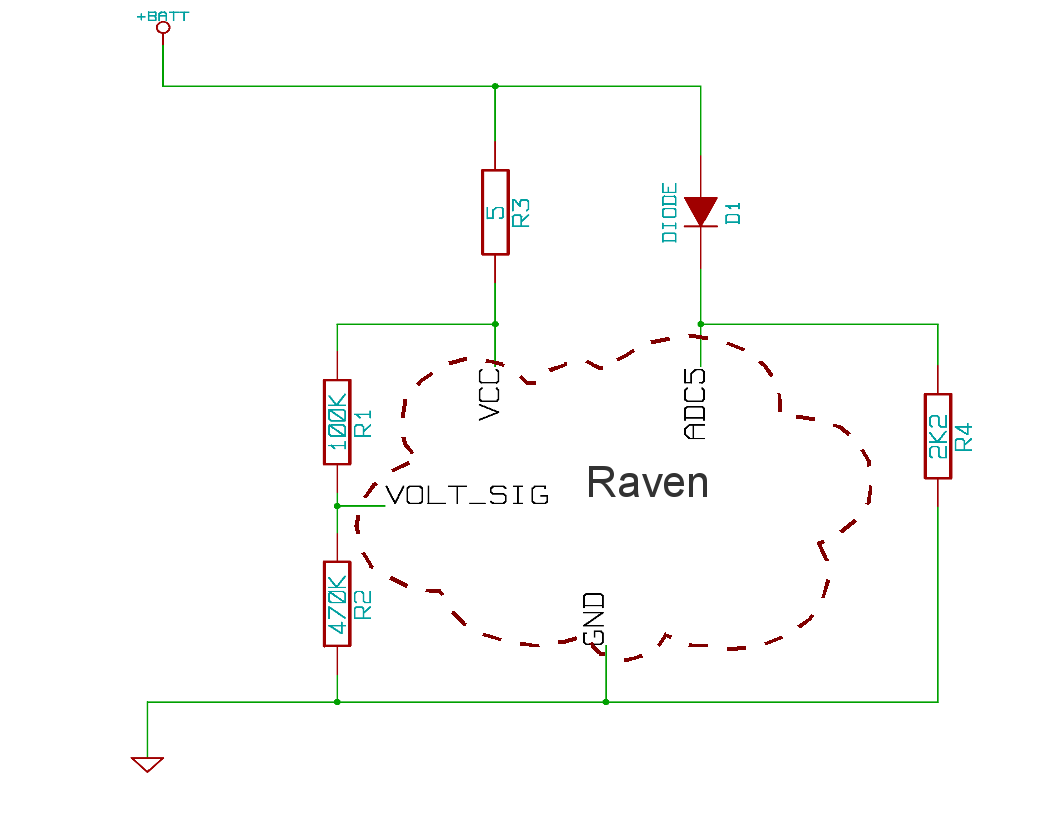
\includegraphics[width=120mm]{static/masurare.png}
 \end{center}
\caption{\small \itshape{Current Measurement setup for the AVR Raven}}

\end{figure}

In order to calculate the instantaneous power used by the sensor node, we need to measure the current flowing from the battery source.
To this end, we connect a shunt resistor in series with the Raven node. Estimating around $30mA$ current, we choose a $5\Omega$ resistor. This
accounts for a voltage drop of about $0.15V$. We would not be able to connect any end of the resistor directly to the ADC, because
if we put the resistor in series, at the GND end of the board, then the GND of the board would not be correct and the voltage
to be measured would be either 0 or negative. If we connect the resistance at the other end, we would surpass VCC, and thus we would not
be able to measure it in the ADC with AVCC reference. Internal reference is no good either, because it is of only $1.1V$. What we 
do is take the voltage at the + end of the resistor and decrease it by 0.5V with the voltage drop of the diode $D1$. To ensure
that $D1$ is opened at all times, we connect it with the GND through the $2.2k\Omega$ resistor $R4$. This ensures the diode is opened
with a minimum $1mA$ flowing. The voltage at the cathode of the diode is measured at an ADC input pin with VCC reference.

\[ADC = f \cdot V_{cc_{board}}\]

\[V_{cc_{real}} - 0.5V = f \cdot V_{cc_{board}},\]
\[V_{cc_{real}} = f \cdot V_{cc_{board}} + 0.5V,\]
$f$ is the ratio given by the ADC, in the range $[0,1]$ with step $\frac{1}{1023}$.
\[V_{cc_{real}} - V_{cc_{board}} =  (f-1) \cdot V_{cc_{board}} + 0.5V\]
\[V_{R_{shunt}} = (f-1) \cdot V_{cc_{board}} + 0.5V\]

We should also calculate precision:

\[ dV_{R_{shunt}} = df \cdot V_{cc_{board}} \]
\[ dI \cdot R = \frac{1}{1023} \cdot V_{cc_{board}} \]
\[ dI = \frac{V_{cc_{board}}}{1023 \cdot 5} ,\]

which for $V_{cc_{board}}$ with values between $1.8V$ and $2.3V$, means precision of $0.39mA$ to $0.45mA$, which we consider
sufficient for our purposes.

The value of the shunt resistor needs to be chosen correctly, a too small value resistor will have a very small voltage drop, 
and precision will be low, a too large value resistor will have a big voltage drop, the sensor node's lifetime will be greatly 
decreased. $0.15V$, as we have chosen, means that the node will have $2.25V$ at full battery (the nodes operates at supply voltages 
greater than $1.8V$)

The voltage and current measurements will be transferred via the inter-processor USART from the Atmega3290 to the Atmega1284. The time interval
in which a Contiki process (associated with a WSN task) is executing is measured, making possible the calculation of the total energy spent
during that interval. This information is then relayed after a specified interval from each of the nodes to the scheduler, who can add them up
and evaluate the schedule.

\section{Algorithm}
\subsection{Formalisation of the problem}

In this subsection we will try to formalise the problem defined in \ref{sec:problem}. First, we will consider the total energy remaining in a
node, $W_{m_k}$, ${m_k}$ being the node. This energy can be deduced from the battery voltage and the discharge profile of the type of battery
used\footnote{ Note however that the Raven Node can only function at voltage over $1.8V$, so $W_{m_k}$ will be the energy remaining until 
the battery provides that threshold voltage.} . We will use this energy, together with the estimated consumption per second, to deduce the 
number of seconds that the node can run. The minimum of these times, calculated over each node in the network, will be the network lifetime.
The purpose of the scheduling algorithm is to maximize this value. 

Because the microcontrollers that we use never enter sleep mode (and their consumption is always very low compared to the transmission/reception
power consumption), we will consider the energy they use incorporated into $W_{idle}$, which can be specific to each node, $W_{idle_{m_k}}$. This
value represents the energy consumed by the sensor node during idle mode in one second. 

\begin{figure}[hb]
\begin{center}
 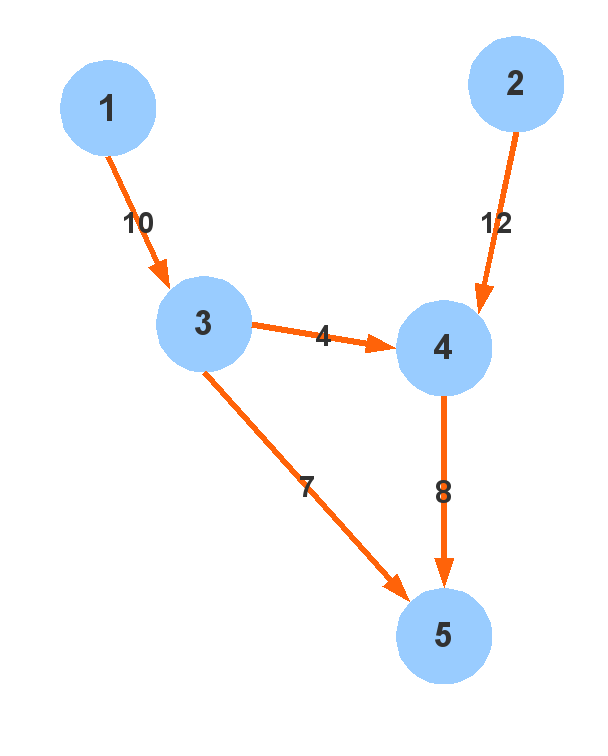
\includegraphics[scale=0.3]{static/dag.png}
\end{center}
\caption{\small \textit{A Directed Acyclic Graph with edges proportional in weight to transmission energy cost.}}

 
\end{figure}

We consider the energy wasted in trasmitting/receiving directly proportional to the number of bits in the payload. To model the tasks and their
dependencies we use a Directed Acyclic Graph (DAG), in which edges represent data dependencies, their cost being the maximal number of bits 
transmitted between the tasks.  (We consider that a transmission occurs after each period). 

Let:
\begin{itemize}
 \item $T(m_k)$ be the set of tasks allocated to node $m_k$.
 \item $W_{idle_{m_k}}$ the idle energy consumed by a node $m_k$ during one second.
 \item $\nu_{i}$ the frequency (in Hz) of the task $v_i$.
 \item $B(e)$, $e\,\in E$, $E$ the set of edges in the task DAG.
 \item $W_{tr\,b,m_k}$,$\,W_{rcv\,b,m_k}$ the energy cost of transmitting/receiving a payload bit on/from node $m_k$.
 \item $M(v)$ is the node to which the task $v$ was assigned.
\end{itemize}

Then the energy consumed by a node $m_k$ is:
\begin{equation}
W_{idle_{m_k}} + \sum_{i,\,v_i\in\,T(m_k)}\:\nu_i(\sum_{j,\,v_j\notin T(m_k)}B(e_{ij}) \cdot W_{tr\,b,m_k}+
\sum_{j,\,v_j\notin T(m_k)}B(e_{ji}) \cdot W_{rcv\,b,m_k})
\end{equation}

Thus the network lifetime is:
\begin{equation}
\max_{k,\,m_k\in M} \frac{W_{m_k}}{\displaystyle
W_{idle_{m_k}} + \sum_{i,\,v_i\epsilon\,T(m_k)}\:\nu_i(\sum_{j,\,v_j\notin T(m_k)}B(e_{ij}) \cdot W_{tr}+
\sum_{j,\,v_j\notin T(m_k)}B(e_{ji}) \cdot W_{rcv})}
\end{equation}

Taking into account that $W_{idle_{m_k}}$ is almost the same on all nodes, and presuming that we have the same amount of energy
available from the batteries, the important part remains the energy consumed in radio transmission. Thus, to maximize network lifetime,
a general goal would be to minimize this consumption. We do not consider tasks that need to be run on all capable nodes, we will 
address this as a restriction in the algorithm.

We have accounted for both energy while transmitting and while receiving. Even if they are not exactly the same, their sum should be uniform
over each bit transmitted, so we can say that the energy consumed by the network in radio communication, $W_{radio}$ is

\begin{equation}
W_{radio} = \sum_{i,j, M(v_i) \neq M(v_j)} B(e_{ij}) * (W_{tr\,b,m_k} + W_{rcv\,b,m_k}) = 
\sum_{i,j, M(v_i) \neq M(v_j)} B(e_{ij}) * K 
\end{equation}

We have reduced the scheduling problem to a known graph-problem, for which a polynomial algorithm has been found in 1988. It is called the
min k-cut problem. If we imagine in our setup the assignment of tasks to nodes, and ascertain that no task is duplicated among nodes
(we can enforce that easily by duplicating in advance tasks that have to be run on all nodes), then the scheduling is in fact a partition of
the node sets $\{C_1,C_2,...,C_k\}$ , each resulting set containing the tasks that have to run on that node. In graph theory, this is called 
a \textit{k-cut}. 

\begin{figure}[ht]
\begin{center}
 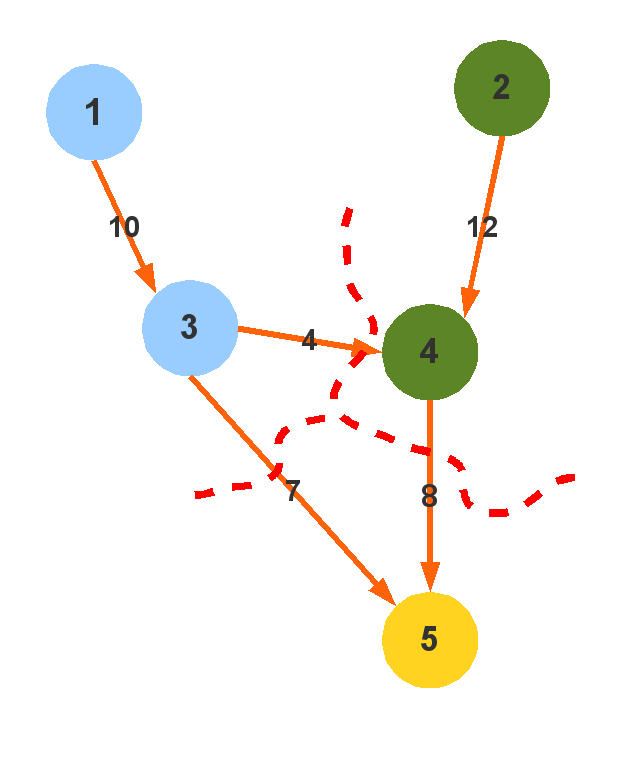
\includegraphics[scale=0.3]{static/dag-cut.png}
\end{center}
\caption{\small \textit{A Directed Acyclic Graph with a minimal 3-way cut. Note that even though on this particular graph the cut is representable in 2D, this
is not always true.}}
\end{figure}

\subsection{Minimal K-Cut}
Given a graph $G=(V,E)$ and a weight function $w:E\rightarrow\mathbb{N}$ and an integer $k\,\in[2..|V|)$ the k-cut is a partition 
of $V$ into $k$ disjoint sets $F=\{C_1,C_2,...,C_n\}$ and its measure is the sum of the weight of the edges between the dijoint sets
\[ \sum_{i=1}^{k-1} \sum_{j=i+1}^{k} \sum_{v_1 \in C_i v_2 \in C_j} w({v_1,v_2}) \]
or otherwise written
\[ \sum_{i,j,\, v_i,v_j\:in\:different\:sets} w({v_1,v_2}) \]

The minimal k-cut algorithm is described in Listing \ref{lst:kcut}
\lstset{numbers=left, mathescape=true, title='SingleCNPT Algorithm', nolol=false,caption=Min K-cut algorithm,label=lst:kcut}
\begin{lstlisting}
KCut(V,k)
  if k is even
    k' = k - 2
  else
    k' = k - 1
  S $\leftarrow$ the set of subsets of k' elements from V
  T $\leftarrow$ the set of subsets of k-1 elements from V

  Find $s\in S,t\in T$ such that W(cut(s,t)) = min
  /* cut(s,t) splits V into s' and t'
  /* Find the minimal cut(s,t) with maximal source set */
  return s' $\bigcup$ KCut(V-s',k-1)
\end{lstlisting}

\subsection{The maximal source minimal s-t cut}

The $(s,t)$ cut, needed by the min K-Cut algorithm, is a partitioning of the vertices of a flow graph such that the source is in $S$ and the 
sink is in $T$. The min K-Cut algorithm needs a version where the source and sink are a set of nodes, not just one. To do this, we can collapse
the nodes in the sink set into a supernode. Edges on the interior of the supernode do not count for the search of the minimal s-t cut, only those
on its exterior. We then proceed to solve the maximum-flow problem on the graph, interpreting weights as flow capacities. Using the residual
graph (graph with edges that have weight the capacity - flux passing at one time), we can start from the sink and expand until we hit 0
residual capacity edges. The nodes found will be the smallest sink set of a minimal s-t cut, the source set being the rest of the nodes. 
\[ r(i,j) = c(i,j) - f(i,j) \]


\lstset{numbers=left, mathescape=true, nolol=false,caption=Maximal source minimal s-t cut,label=lst:stcut}
\begin{lstlisting}
mstCut(S,T)
  /* replace sink and source set by supernodes */
  $V'=V \bigcup \{s,t\} - (S \bigcup T)$
  modify the edges external to supernodes
  $E'=\{e_{ij}|i,j\notin S,T\}\bigcup \{e_{si}|e_{ji}\in E\,and\,j\in S\} \bigcup$
  $\{e_{ti}|e_{ji}\in E\,and\, j \in T\} \bigcup \{e_{st}|e_{ij}, i \in S, j \in T\}$
  $F_{ij}=0,\,\forall i,j\in V$
  while 1
    find path $p$ from $s$ to $t$ in residual graph
    $m \leftarrow$ minimum residual capacity on path $p$
    for each edge $e_{ij}$ on path $p$
      $F_{ij} \leftarrow F_{ij} + m$
      $F_{ji} \leftarrow F_{ji} - m$

  $A \leftarrow$ set of nodes reachable by BFS from $t$
  $B \leftarrow V-A$
  return $(A,B)$
\end{lstlisting}



\subsection{Adaptation of K-Cut}
\label{sec:adapt} 

When reducing the scheduling problem to K-Cut, some constraints were ignored that now must satisfied. Since every step of the alghoritm is
partitioning the node set in half, one being final and one remaining to be further partitioned, we can say that each step represents scheduling
tasks on a single node. Contraints must be inserted in each step, relevant to the node whose tasks are being scheduled. In the pseudocode of
the algorithm, finding the source set $S$ is what must be modified to satisfy constraints.

We have several constraints that must be added to the algorithm:
\begin{itemize}
 \item Some tasks can only run on compatible nodes
 \item Some tasks have to run on all capable nodes (e.g. sensing tasks)
\end{itemize}

\begin{figure}[ht]
 \begin{center}
  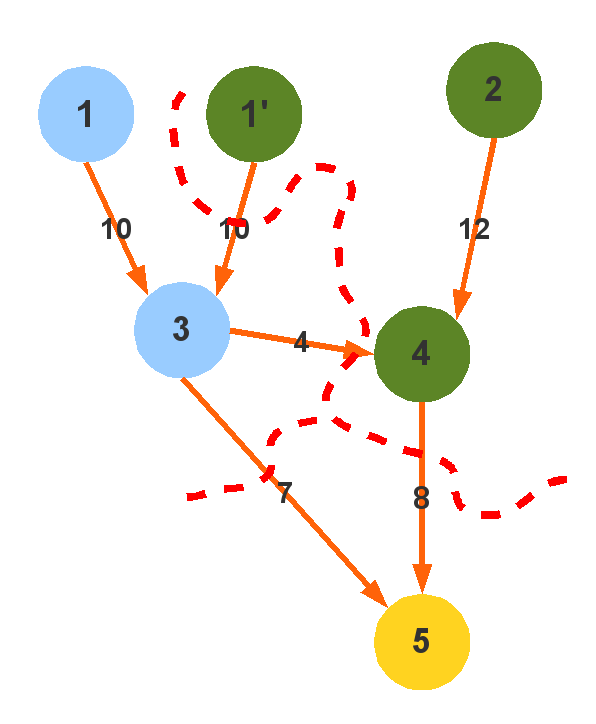
\includegraphics[scale=0.3]{static/dag-cut-multiplier.png}
 \end{center}
 \caption{\small \itshape{A directed graph with a task that has to be duplicated on all capable nodes}}
\end{figure}

To enforce the first constraint we have to include only compatible tasks (tasks $v$ such that $NA(v,m)=1$ for the current node $m$) in 
the source set, as well as filter the cuts in which the first resulting set contains incompatible tasks. For the second constraint, 
we will include the tasks that have to be duplicated in the sink set of the cut (so that they will be available for the next step 
of the algorithm), then in the end we add those tasks to those obtained in the minimal $(s,t)$ cut.
\lstset{numbers=left, mathescape=true, nolol=false,caption=Adapted min K-Cut,label=lst:mkcut}
\begin{lstlisting}
MKCut(V,k,$m_i$)
  if k is 
    k' = k - 2
  else
    k' = k - 1
  MT $\leftarrow$ {tasks that have multiplicity}
  V' $\leftarrow$ V - MT
  S $\leftarrow$ {the set of subsets of k' elements from V'}
  T $\leftarrow$ {the set of subsets of k-1 elements from V'}$ \bigcup$ MT

  Find $s\in S,t\in T$ such that W(cut(s,t)) = min
  /* cut(s,t) splits V into s' and t'
  /* Find the minimal cut(s,t) with maximal source set */
  $T(m_i) = \{s'\}\bigcup \{v_j| v_j \in $ MT$, NA(v_j,m_i)=1\}$
  return $T(m_i)\,\bigcup$ KCut(V-s',k-1,$m_{i+1}$)
\end{lstlisting}

Assigning the tasks for each node at each step gives great versatility in constraints management for the algorithm to better model and
solve the problem. For instance, battery status has no role yet, but it is easy to add: We set a threshold for the battery/tasks ratio,
if the current node crosses that threshold we will settle on another solution, not necessarily with the same min k-cut, but with less
strain on the node.

\subsection{Complexity}

The complexity of the min k-cut with the algorithm we described is:
\[T(n) = O(n^{k'+k+1}) \cdot O(n^3) + T(n-1), \]

where $O(n^3)$ is the bound for the minimum (s,t)-cut algorithm.

For $k$ even, we have:

\[O(n^{2k-3}(n^3 + n^{2k-4}(n^3 + ... n^4(n^3 + n^3)))))) = O (n^{k^2})\]

A precise evaluation gives, as found by \cite{Gold1988}:

\[O(n^{k^2 - 3k/2 + 2}),\:k\,even \]
\[O(n^{k^2 - 3k/2 + 5/2}),\:k\,odd \]

\section{Approximation Alternative}
\subsection{Gomory-Hu trees}

We will construct then \textit{Gomory-Hu} trees (or cut trees). From those we will deduce the cut with minimal weigth and
maximal source set needed for our scheduling algorithm.

Let $G=(V,E)$ be a graph and $c:E\rightarrow\mathbb{R}$ a cost function for its edges. Let $T$ be a tree with the node set $V$, and $c'$ a
cost function for edges in $T$. Then the $T$ is a Gomory-Hu tree for $G$ if:
\begin{itemize}
 \item $\forall\,s,t\in V$, the cost of the minimum $s-t$ cut in $G$ coincides with the cost of the minimum $s-t$ cut in $T$.
 \item $\forall$ edges $\,[s,t]\in\,T$, $c'(x,y)$ is the cost of the minimum $s-t$ cut in $G$.
\end{itemize}

\begin{figure}[ht]
\begin{center}
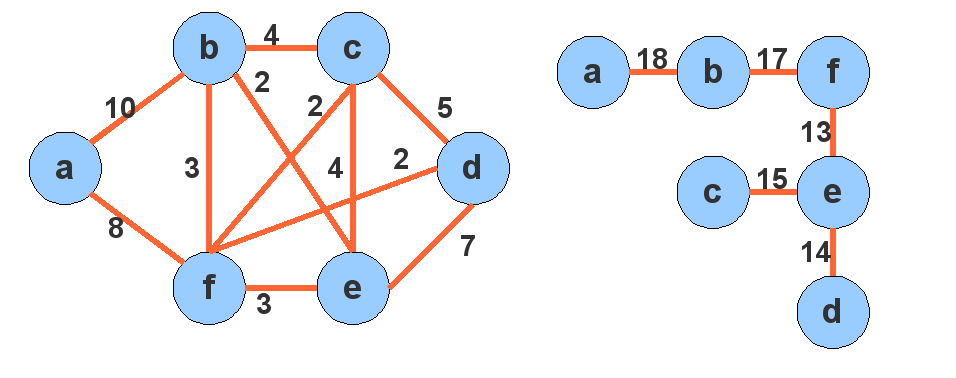
\includegraphics[scale=0.4]{static/gomory-hu.png}
\end{center}
\caption{\small \itshape{A graph (left) and its Gomory-Hu tree (right) }}
\end{figure}

\subsection{Approximation Algorithm}

The algorithm is based on a theorem from \cite{Jaco2006}:

\textit{Removing l cuts associated with l edges in the Gomory-Hu tree for G results in a new graph G'
with at least l+1 connected components.}

The idea behind the algorithm is to build the Gomory-Hu tree of graph $G$, named $T$. We will take the 
lightest $k-1$ cuts from the $n-1$ cuts associated with the graph $G$, leaving at least $k$ components.

\section{Integration in SENSEI}

In the SENSEI project, the scheduling algorithm presented here appears under \textit{Check - Scheduling for Task-based WS\&ANs}. It is
implemented as a service available through multiple interfaces, some standard SENSEI interfaces and some non-standard. 

\begin{figure}[ht]
\begin{center}
 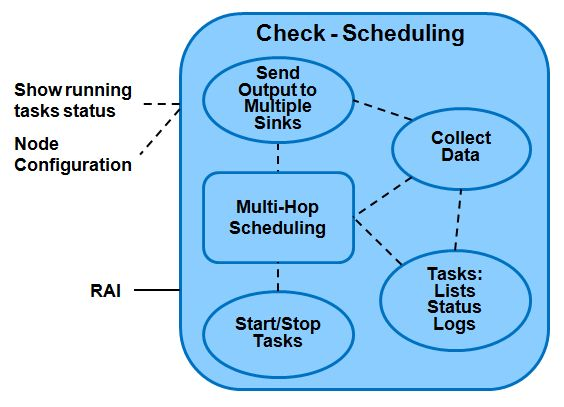
\includegraphics[width=90mm]{static/check.png}
\end{center}
\caption{\small \itshape{Check - Scheduling as a SENSEI Building Block}}
\end{figure}

RAI is a standard SENSEI interface (stands for Resource Access Interface), that will enable access to the different functionalities 
of the WS\&AN island:
\begin{itemize}
\item \textit{Collecting Data} - RAI.get(``parameters'') would gather sensor data.
\item \textit{Starting/Stopping tasks} - RAI.set(``start'') or RAI.set(``stop'') would start or stop tasks in a WS\&AN island. This is tied to
the dynamic scheduling functionality.
\item \textit{Sending Output to Multiple Sinks} - This is automatically taken care of if a task has several succesors in a data-dependency
graph of the application.
\item \textit{Tasks: List,Status,Logs} - Allows for monitoring the island, generating statistics or investigation of failures.
\item \textit{Multi-hop Scheduling} - Extension of the algorithm for multi-hop situations.
 ×
\end{itemize}

As shown in Figure \ref{fig:dep}, Check Scheduling has a couple of dependencies in the SENSEI project, one is from the Connectivity domain,
multi-hop routing, the other is related to Management of WSNs, Reprogramming, Monitoring and Self-healing. In the figure, blue
represents middleware (The Check-Scheduling Algorithm is considered to be a middleware component), pink stands for management and
yellow for connectivity. 

Multi-hop routing is needed to extend the algorithm to a network with graph topology. Reprogramming Over-the-Air (OTA) is needed for
faster development, Monitoring is related to the data that Check - Scheduling exposes through the RAI interface and the Self-healing would be
one of the services that uses the Check-scheduler, reconfiguring the tasks around the WS\&AN island to replace node failures in the WSN network.
\begin{figure}[ht]
\begin{center}
 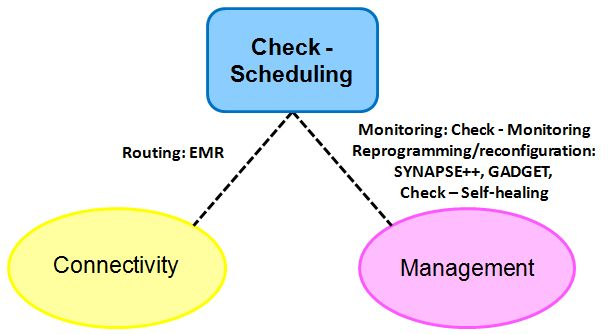
\includegraphics[width=90mm]{static/check2.png}
\end{center}
\caption{\small \itshape{Check - Scheduling Dependencies}}
\label{fig:dep}
\end{figure}